
%TODO:Анализ результатов
\chapter{ВЫЧИСЛИТЕЛЬНЫЙ ЭКСПЕРИМЕНТ}
%\section{Вычислительный эксперимент}

Основным вопросом, поставленным в данной работе является нахождение таких состояний системы трех тел, что внутренняя энергия, запасенная в пружинах будет максимальна или минимальна. А так же нахождение таких состояний, при которых внутренняя энергия тела после соударения равна 0 или же наоборот вся вся кинетическая энергия перейдет во внутреннюю.

Для нахождения потерь энергии во время взаимодействия запишем Закон сохранения энергии:
\begin{equation}\label{eq:energy}
    \frac{M v_0^2}{2} = \frac{m_1 v_1^2}{2} + \frac{m_2 v_2^2}{2} + \frac{m_3 v_3^2}{2} + \frac{k_2 \Delta l^2}{2} + \frac{k_3 \Delta l^2}{2}
\end{equation}, где $M = m_1 + m_2 + m_3$. Энергия, накопленная первой пружиной отсутствует, так как вся энергия пружины переходит в ускорение тел и растяжение и сжатие остальных пружин.

Так как нас интересует потери энергии для тела на макроуровне, то рассмотрим систему трех тел после соударения как единое тело с постоянной скоростью, тогда разница между кинетическими энергиями до и после соударения и будет показывать накопленную внутреннюю энергию тела. Для этого запишем уравнение для скорости центра масс:

\begin{equation}
    v_c = \frac{m_1 v_1 + m_2 v_2 + m_3 v_3}{M}
\end{equation}
, тогда Закон сохранения энергии примет вид:

\begin{equation}
    \frac{M v_0^2}{2} = \frac{M v_c^2}{2} + \Delta E
\end{equation}
, где $\Delta E$ - энергия накопленная в пружинах и кинетическая энергия движения масс относительно центра масс.


\begin{figure}[b!]
    \centering
    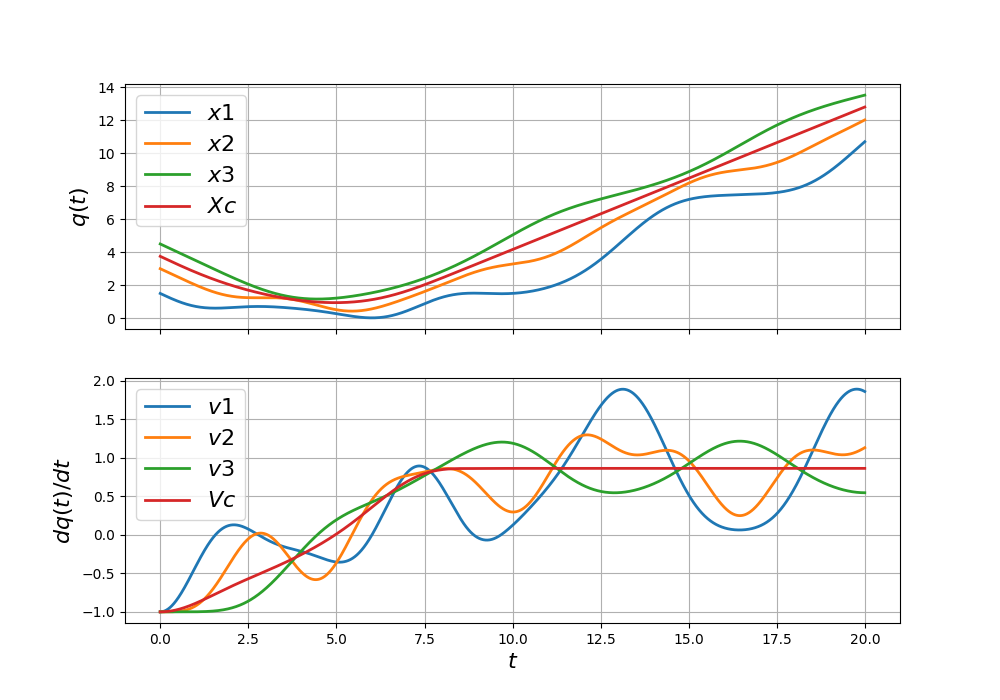
\includegraphics[width=0.7\textwidth]{snaps_midd.png}
    \caption{График координат и скоростей тел на микроуровне и на макроуровне(красным).}
    \label{fig:snapmidd}
\end{figure}

На рисунке \ref{fig:snapmidd} на графике продемонстрирован результат симуляции с нахождением скорости центра масс, а так же его координат, из чего можно сделать вывод что после взаимодействия часть кинетической энергия тела перешла во внутреннюю энергию тела, соответственно скорость тела после соударения уменьшилась. Массы для данной симуляции заданы следующим образом: $m_1 = m_2 = 1; m_3 = 4$. Начальная скорость $v_0$=1м/с. При этом можно увидеть, что итоговая скорость тела после взаимодействия меньше первоначальной, засчет преобразования энергий. Энергия, перешедшая во внутреннюю и есть искомая $\Delta E$.

Проведем вычислительный эксперимент с различными входными параметрами системы (длина пружин $l=1$). Для определения параметра, в большей степени влияющего на состояние системы измерим $\Delta E$ для каждого параметра в некоторых пределах. Но очевидно что, например, большая масса способна сильней повлиять на численное значение $\Delta E$. Тогда введем $\Delta \tilde{E} = \frac{\Delta E}{E_0}$, где $E_0$ - изначальная энергия системы. $\Delta \tilde{E}$ - коэффициент эффективности диссипации энергии. Для случая представленного на рисунке \ref{fig:snapmidd} $\Delta \tilde{E} = 27.26\%$. На графиках на рисунке \ref{fig:deltas} продемонстрированы зависимость коэффициента эффективности диссипации от различных масс.


\begin{figure}[b!]
    \centering
    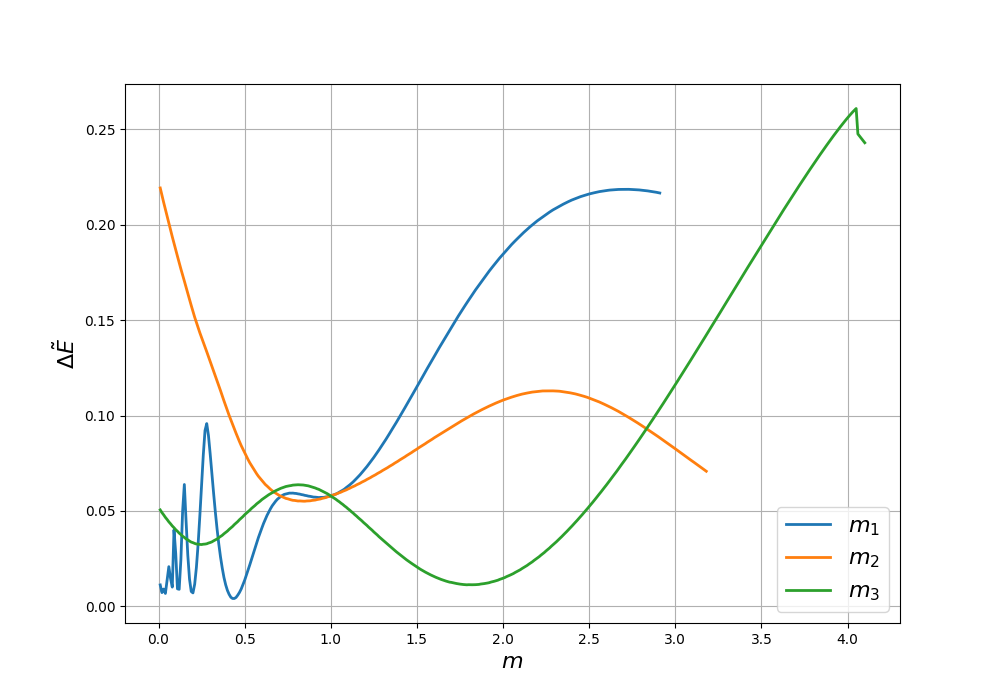
\includegraphics[width=0.7\textwidth]{deltas.png}
    \caption{Зависимость $\Delta \tilde{E}$ от различных значений масс. Каждый график соответствует одной переменной массе.}
    \label{fig:deltas}
\end{figure}

Аналогичный эксперимент проведем для переменных жесткостей пружин:

\begin{figure}[b!]
    \centering
    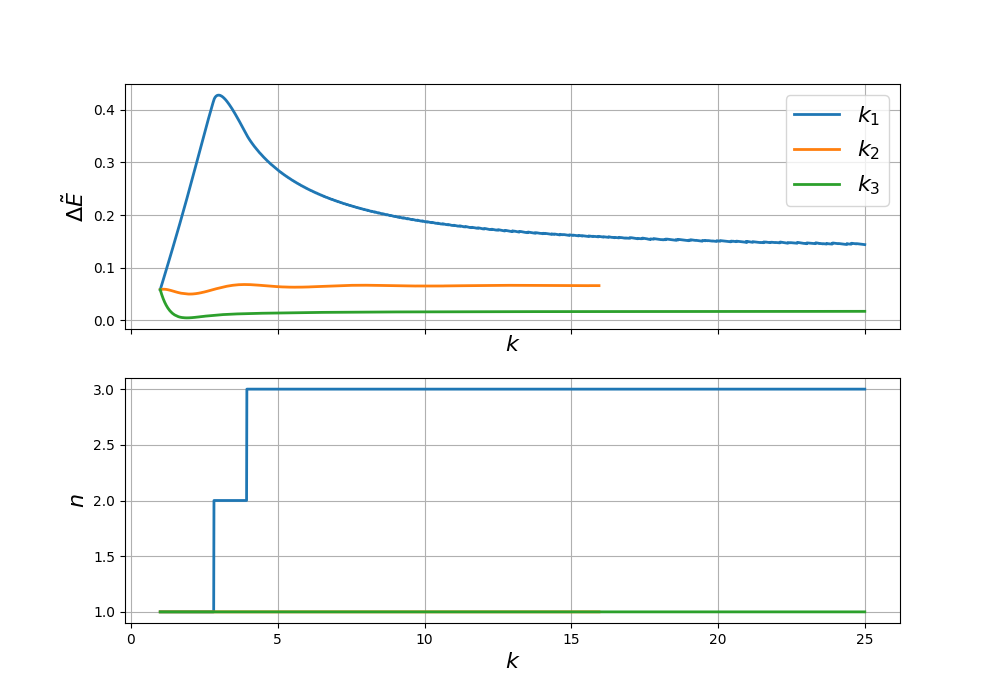
\includegraphics[width=0.7\textwidth]{stiff_deltas.png}
    \caption{Зависимость $\Delta \tilde{E}$ от различных значений жесткости пружин. Каждый график соответствует одной переменной массе. Нижний график демонстрирует зависимость количества соударений со стенкой от жесткости.}
    \label{fig:stiff_deltas}
\end{figure}

На первом графике на рисунке \ref{fig:stiff_deltas} видно, что $\Delta \tilde{E}$ сильнее всего зависит от значения жесткости первой пружины. При этом значение $\Delta \tilde{E}$ линейно достигает максимума, а затем логарифмически убывает. На нижнем графике продемонстрировано количество ударов о стенку в зависимости от жесткости пружины, важно заметить, что количество соударений зависят только от жесткости $k_1$. На основе рисунка \ref{fig:stiff_deltas}  можно сделать вывод, что максимальные значения $\Delta \tilde{E}$ находятся при значении $n=2$. При этом можно заметить, что значение жесткости $k_2$ практически не влияет на состояние системы, а увеличение значения жесткости $k_3$, наоборот приводят к уменьшению $\Delta \tilde{E}$, а следовательно и накопленной системой энергии.

Рассмотрим поведение системы для двух переменных параметров, для определения значений $\Delta \tilde{E}$.
Для этого построим срезы по различным плоскостям шестимерного пространства значений $k_1 k_2 k_3 m_1 m_2 m_3$. 
Белые области на графиках обозначают нефизические случаи. Для того чтобы избавиться от нефизических случаев было решено увеличить длну пружин и 
принять ее значение $l=10$.

\begin{figure}[b!]
    \begin{minipage}[h]{0.5\linewidth}
        \center{
            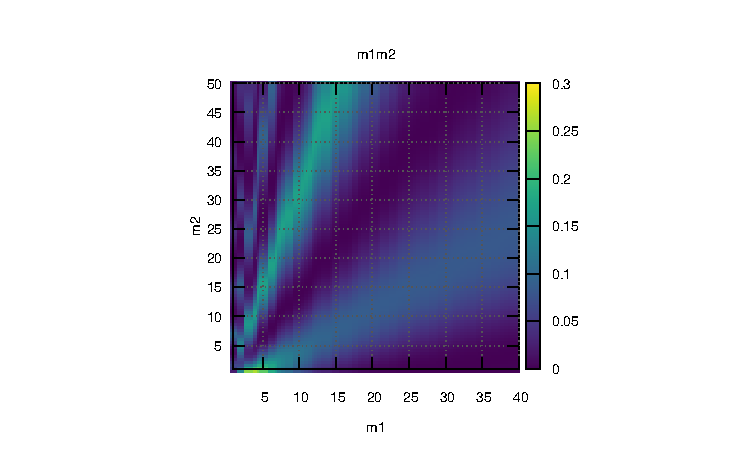
\includegraphics[width=1\textwidth]{m1m2.pdf} \\ a)
        }
    \end{minipage}
    \hfill
    \begin{minipage}[h]{0.5\linewidth}
        \center{
            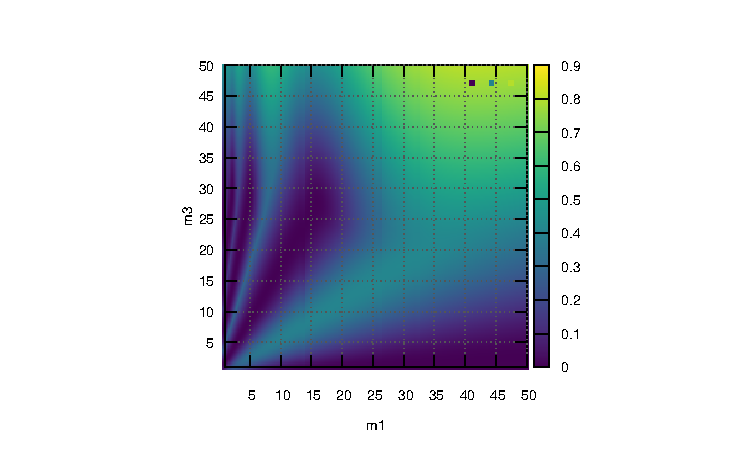
\includegraphics[width=1\textwidth]{m1m3.pdf} \\ б)
        }
    \end{minipage}
    \begin{center}
        \begin{minipage}[h]{0.5\linewidth}
            \center{
                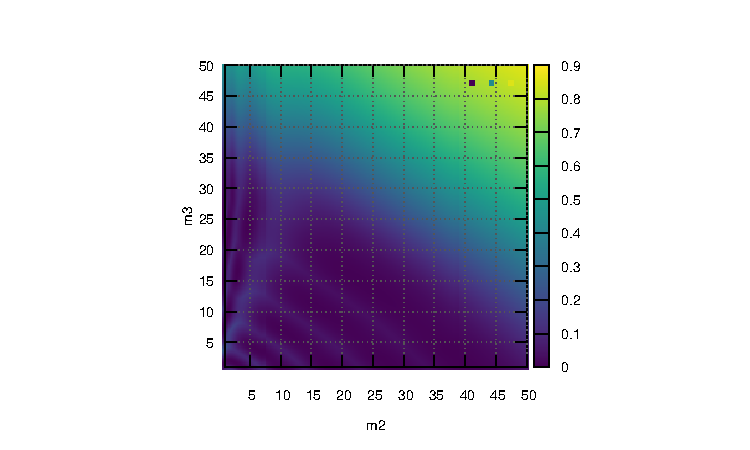
\includegraphics[width=1\textwidth]{m2m3.pdf} \\ в)
            }
        \end{minipage}
    \end{center}
    \caption{Срезы значений $\Delta \tilde{E}$ для двух переменных масс: $m_1$ $m_2$ (а), $m_1$ $m_3$ (б), $m_2$ $m_3$ (в). $l =10$ Фиксированные жесктости и массы =1}
    \label{fig:var2mass}
\end{figure}

\begin{figure}[b!]
    \begin{minipage}[h]{0.5\linewidth}
        \center{
            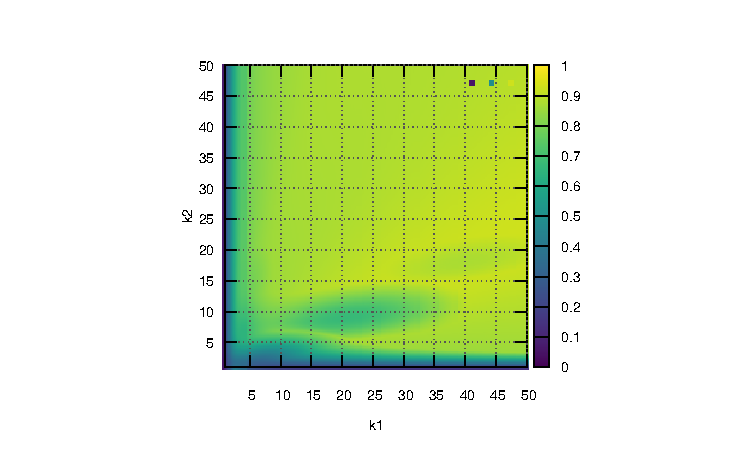
\includegraphics[width=1\textwidth]{k1k2.pdf} \\ a)
        }
    \end{minipage}
    \hfill
    \begin{minipage}[h]{0.5\linewidth}
        \center{
            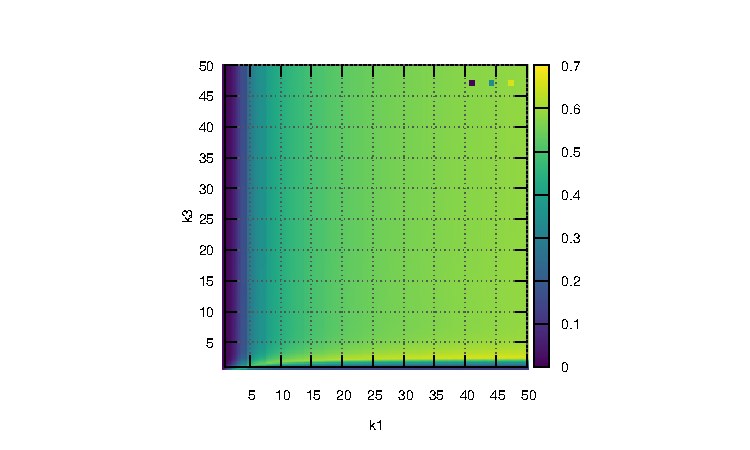
\includegraphics[width=1\textwidth]{k1k3.pdf} \\ б)
        }
    \end{minipage}
    \begin{center}
        \begin{minipage}[h]{0.5\linewidth}
            \center{
                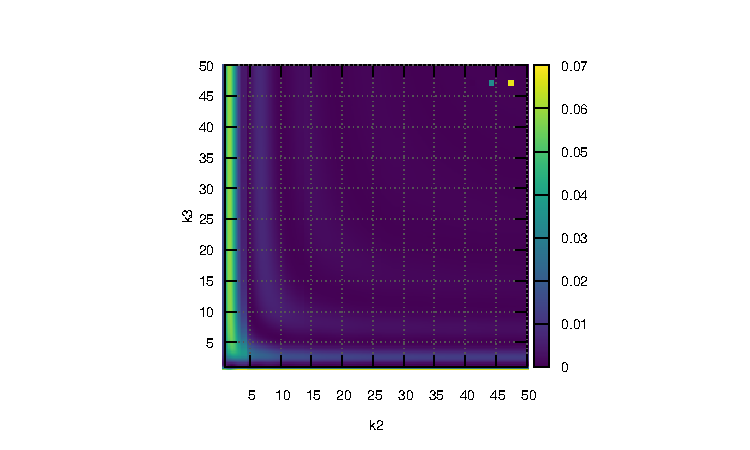
\includegraphics[width=1\textwidth]{k2k3.pdf} \\ в)
            }
        \end{minipage}
    \end{center}
    \caption{Срезы значений $\Delta \tilde{E}$ для двух переменных жесткостей: $k_1$ $k_2$ (а), $k_1$ $k_3$ (б), $k_2$ $k_3$ (в). $l =10$ Фиксированные жесткости и массы =1}
    \label{fig:var2stiff}
\end{figure}



\begin{figure}[b!]
    \begin{minipage}[h]{0.3\linewidth}
        \center{
            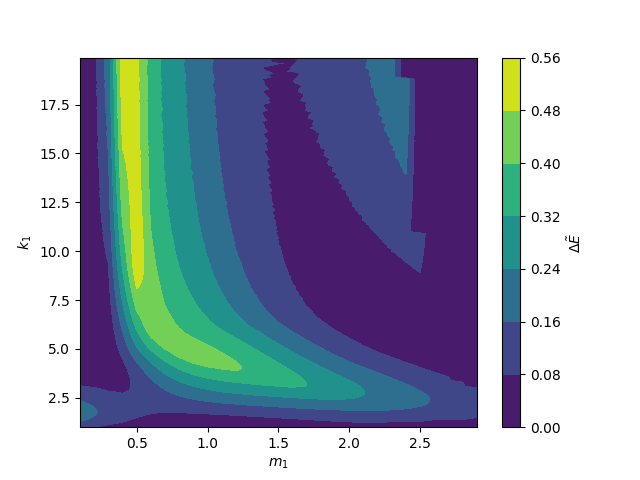
\includegraphics[width=1\textwidth]{m1k1.png} \\ a)
        }
    \end{minipage}
    \hfill
    \begin{minipage}[h]{0.3\linewidth}
        \center{
            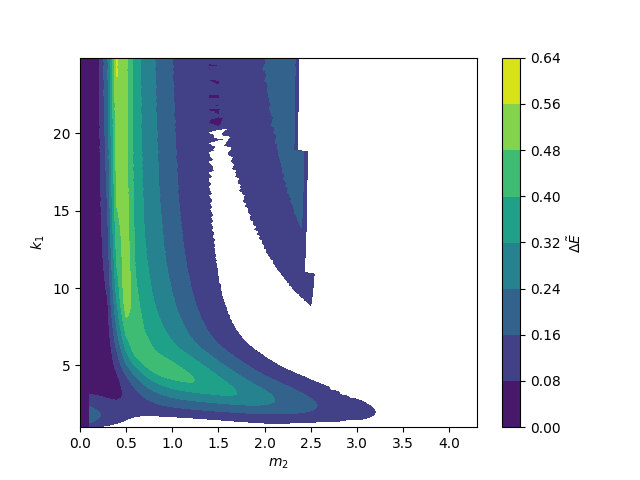
\includegraphics[width=1\textwidth]{m2k1.png} \\ б)
        }
    \end{minipage}
    \begin{minipage}[h]{0.3\linewidth}
        \center{
            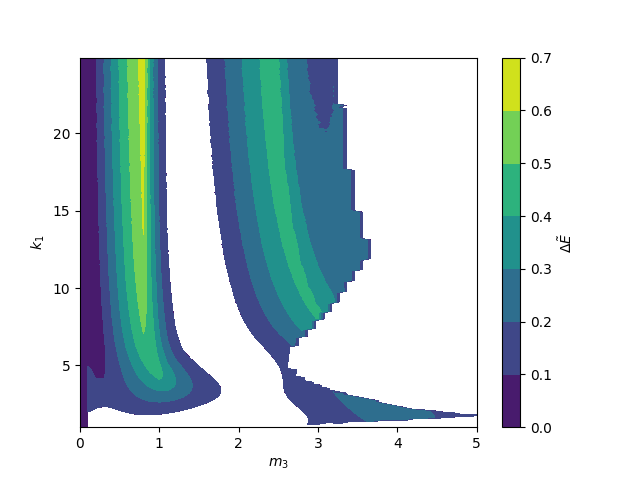
\includegraphics[width=1\textwidth]{m3k1.png} \\ в)
        }
    \end{minipage}
    \caption{Срезы значений $\Delta \tilde{E}$ для переменной жесткости $k_1$ и переменной массы: $m_1$ (а), $m_2$ (б), $m_3$ (в)}
    \label{fig:var2k1}
\end{figure}


\begin{figure}[b!]
    \begin{minipage}[h]{0.3\linewidth}
        \center{
            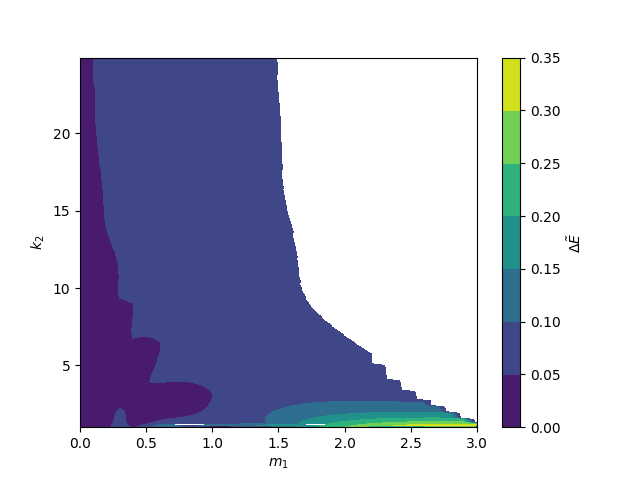
\includegraphics[width=1\textwidth]{m1k2.png} \\ a)
        }
    \end{minipage}
    \hfill
    \begin{minipage}[h]{0.3\linewidth}
        \center{
            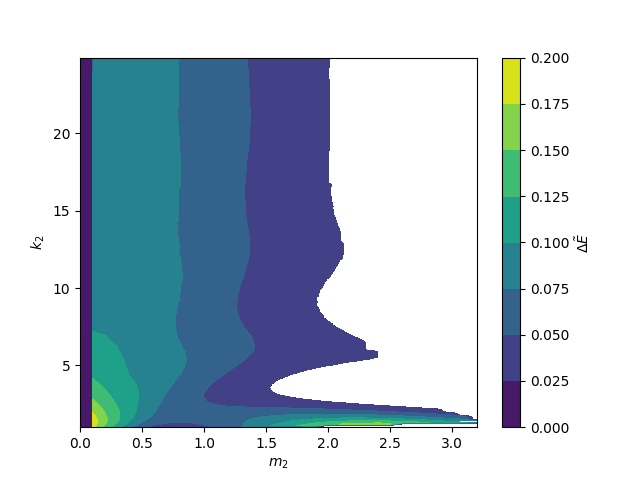
\includegraphics[width=1\textwidth]{m2k2.png} \\ б)
        }
    \end{minipage}
    \begin{minipage}[h]{0.3\linewidth}
        \center{
            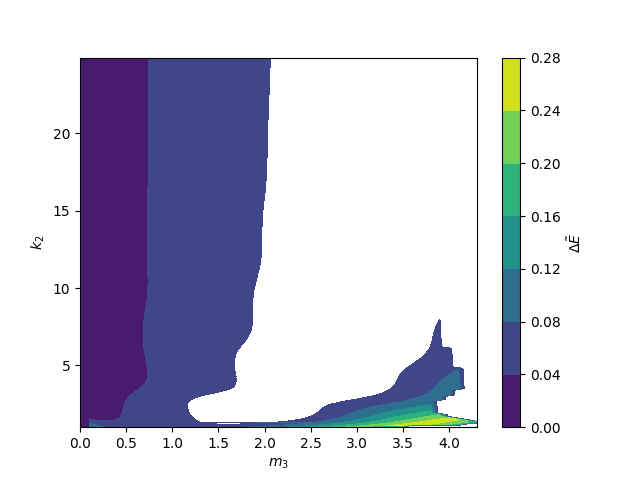
\includegraphics[width=1\textwidth]{m3k2.png} \\ в)
        }
    \end{minipage}
    \caption{Срезы значений $\Delta \tilde{E}$ для переменной жесткости $k_2$ и переменной массы: $m_1$ (а), $m_2$ (б), $m_3$ (в). Цветом обозначена величина накопленной энергии}
    \label{fig:var2k2}
\end{figure}


\begin{figure}[b!]
    \begin{minipage}[h]{0.3\linewidth}
        \center{
            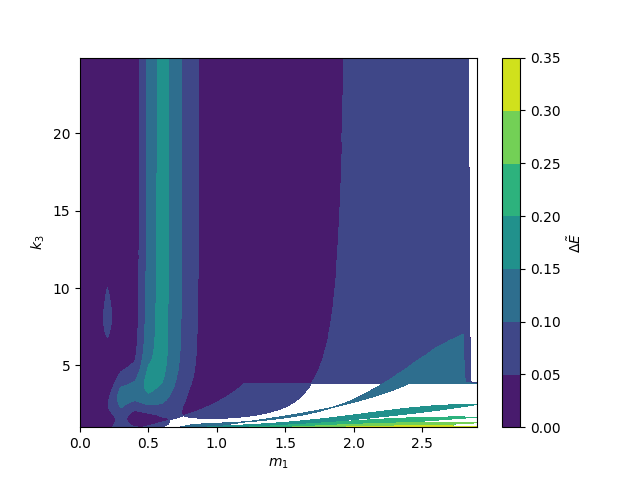
\includegraphics[width=1\textwidth]{m1k3.png} \\ a)
        }
    \end{minipage}
    \hfill
    \begin{minipage}[h]{0.3\linewidth}
        \center{
            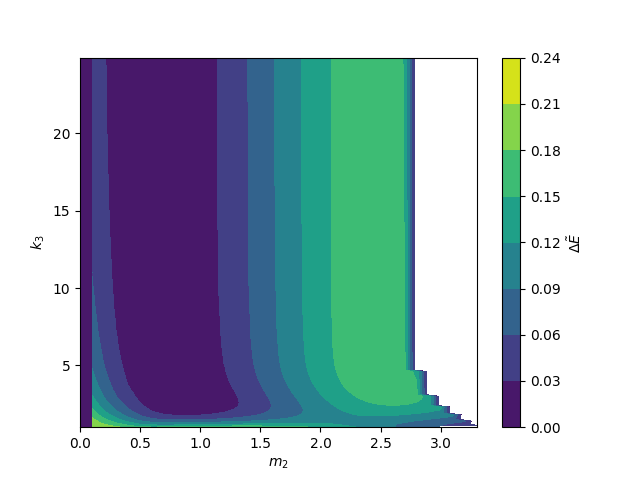
\includegraphics[width=1\textwidth]{m2k3.png} \\ б)
        }
    \end{minipage}
    \begin{minipage}[h]{0.3\linewidth}
        \center{
            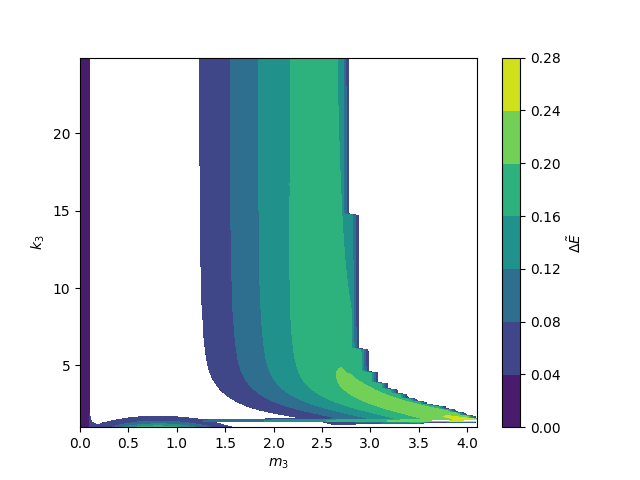
\includegraphics[width=1\textwidth]{m3k3.png} \\ в)
        }
    \end{minipage}
    \caption{Срезы значений $\Delta \tilde{E}$ для переменной жесткости $k_3$ и переменной массы: $m_1$ (а), $m_2$ (б), $m_3$ (в). }
    \label{fig:var2k3}
\end{figure}


Полученные срезы позволяют понять какие переменные вносят больший вклад в диссипацию энергии в системе. Но данная выборка не может считаться полностью репрезентативной, так как в большинстве случаев области значений подобраны таким образом чтобы ограничить область нефизических случаев. Но даже такие данные позволяют сделать некоторые выводы насчет поведения системы. В частности на рисунке \ref{fig:var2mass} можно увидеть периодичность максимумов, при этом для графиков (a) и (б) она зависит от $tg \alpha$ равное соотношению масс. Для графика (в), область оптимальных значений находится в области $m_3 \rightarrow min$, но в то же время максимумы чередуются в зависимости от значения $m_2$. Что позволяет сделать вывод, о том что $\Delta \tilde{E}$ зависит в большей степени не от значений масс системы, а от их отношения.

При этом если рассматривать графики, изображенные на рисунке \ref{fig:var2stiff}, то можно легко заметить по графикам (а) и (б), что
$\Delta \tilde{E}$ практически не зависит от значений $k_2$ и $k_3$, но при этом линейно зависят от значений $k_1$. Основной вклад в диссипацию энергии вносит первая пружина, а на по графику (в) видно что при минимизации жесткости $k_2$ происходит увеличение $\Delta \tilde{E}$, что соответствует данным, полученным на графике (а).

На рисунке \ref{fig:var2k1} можно увидеть, что $\Delta \tilde{E} \rightarrow max$ при определенных значениях массы и линейно зависят от $k_1$ в окрестностях оптимальной массы. Так же можно предположить некоторую периодичность процесса, но по причине того, что для данных переменных, система достаточно быстро переходит в нефизическое состояние, то делать сложно делать какие либо однозначные выводы.

Рисунки  \ref{fig:var2k2} и \ref{fig:var2k3} демонстрируют зависимость $\Delta \tilde{E}$ для переменных масс и жесткостей $k_2$ и $k_3$ соответственно. Но легко можно заметить, что максимальные значения $\Delta \tilde{E}$ находятся на границе с нефизическими состояниями системы. Скорей всего данные отношения не представляют какой либо практический интерес.

Контуры срезов, полученные на рисунках \ref{fig:var2mass} - \ref{fig:var2k3} соответствуют данным, полученным на рисунках \ref{fig:deltas} и \ref{fig:stiff_deltas}. На графиках присутствует периодичность для масс, которую можно заметить и на полученных срезах, а так же видна линейная зависимость $\Delta \tilde{E}$ от $k_1$.

Рассмотрим трехмерные пространства изменяемых параметров масс и жесткостей пружин. Для этого провердем численный эксперимент для каждого значения массы
с выбранным шагом($h=0.5$), и получим облака точек, изображенные на рисунке \ref{fig:3d}, значения накопленной энергии в которых, обозначено цветом.


\begin{figure}[b!]
    \centering
    \begin{minipage}[h]{0.49\linewidth}
        \center{
           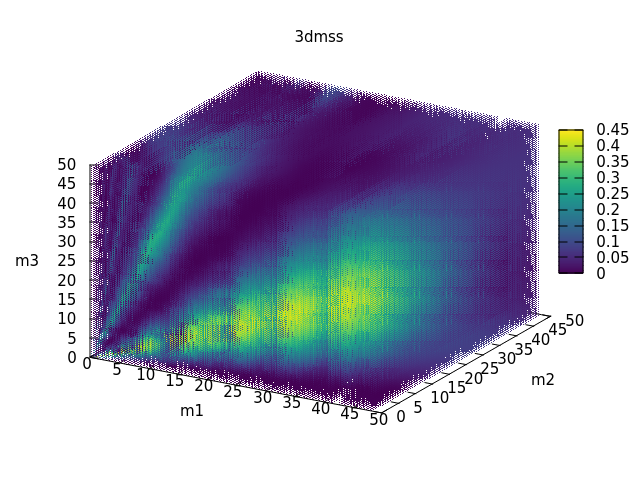
\includegraphics[width=1\textwidth]{3dmssnew.png} \\ a)
        }
    \end{minipage}
    \hfill
    \begin{minipage}[h]{0.49\linewidth}
        \center{
           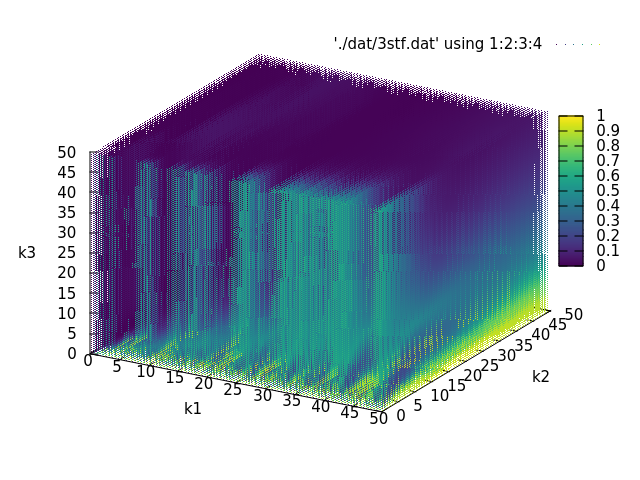
\includegraphics[width=1\textwidth]{3dstfs.png} \\ б)
        }
    \end{minipage}
    \caption{Зависимость $\Delta \tilde{E}$ от различных значений масс (a) и различных значений жесткостей (б). Значение $\Delta \tilde{E}$ указано цветом.}
    \label{fig:3d}
\end{figure}

Так как сами по себе графики представленные на рисунке \ref{fig:3d} не очень репрезентативны, то построим графики содержащие только точки в которых значение $\Delta \tilde{E} < 0.01$. 
точек, отображающие зоны минимальных и максимальных накопленных энергий. 

\begin{figure}[b!]
    \centering
    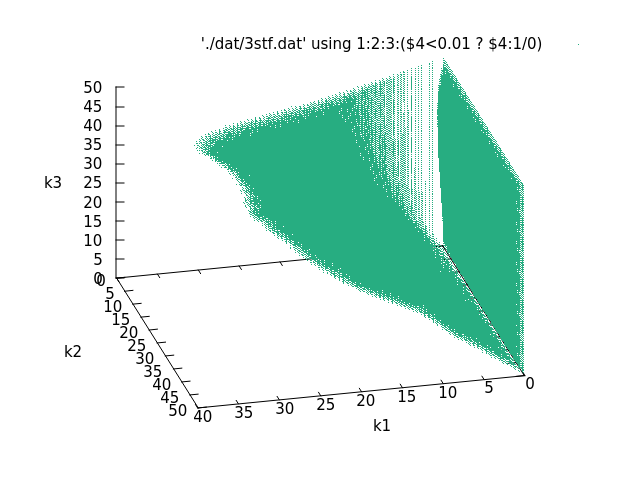
\includegraphics{stfsmin.png}
    \caption{Области $\Delta \tilde{E} < 0.01$  для переменных жесктостей}
    \label{minmss3d}
\end{figure}


\begin{figure}[b!]
    \centering
    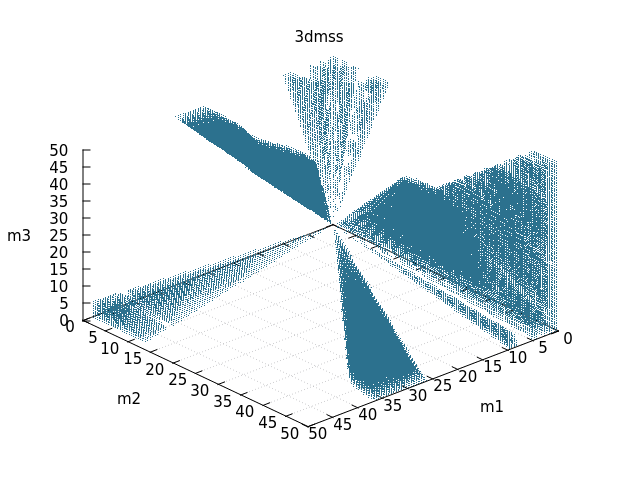
\includegraphics{3dmssmin.png}
    \caption{Области $\Delta \tilde{E} < 0.01$  для переменных масс}
    \label{minmss3d}
\end{figure}

\begin{figure}[b!]
    \centering
    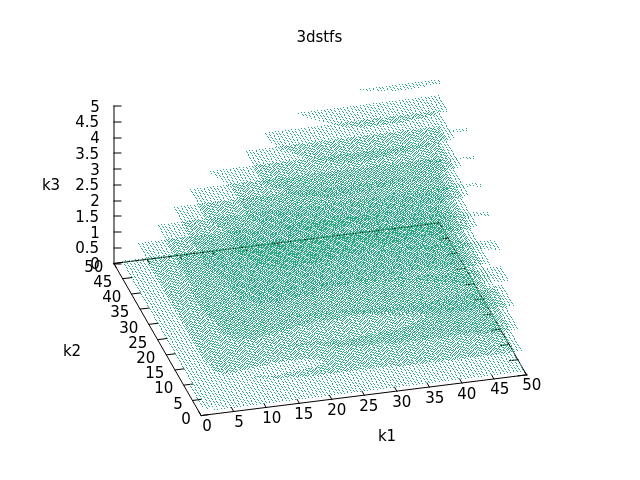
\includegraphics{3dstfsmax.png}
    \caption{Области максимальных значений $\Delta \tilde{E}$  для переменных жесткостей}
    \label{minmss3d}
\end{figure}

\newpage
\begin{figure}[b!]
    \centering
    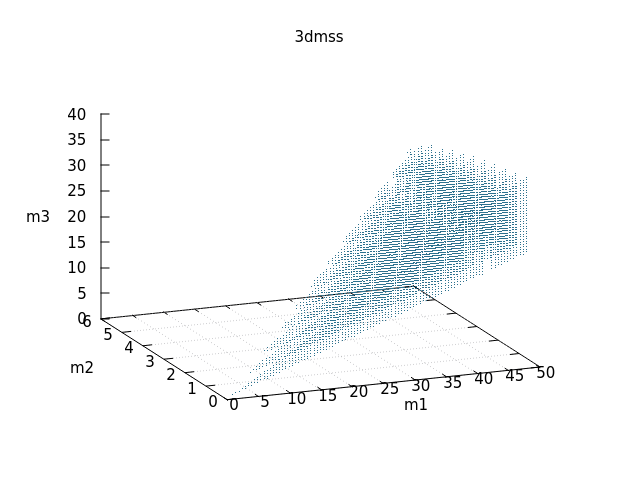
\includegraphics{3dmssmax.png}
    \caption{Области максимальных значений $\Delta \tilde{E}$  для переменных масс}
    \label{minmss3d}
\end{figure}

Посторим траектории системы трех тел в полученных областях максимальных и минимальных энергий. Полученные траектории могут продемонстрировать механизмы перехода
энергии с макроуровня на микроуровень.

%\begin{figure}[t!]
%    \centering
%    \centering
%    \begin{minipage}[h]{0.49\linewidth}
%        \center{
%           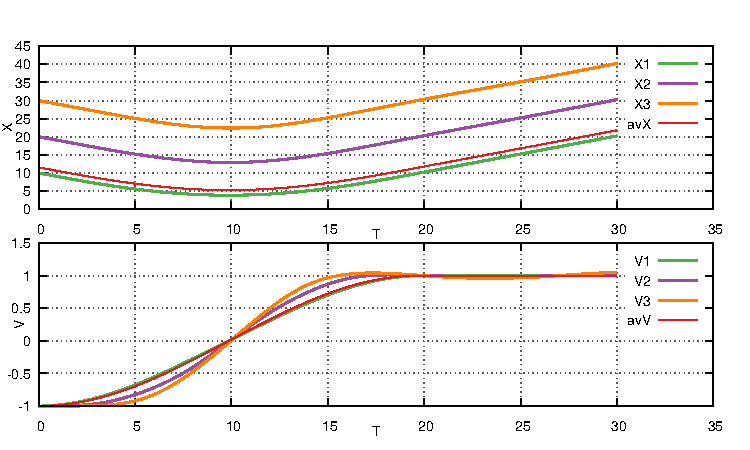
\includegraphics[width=1\textwidth]{tr/trbigm1.pdf} \\ a)
%        }
%    \end{minipage}
%    \hfill
%    \begin{minipage}[h]{0.49\linewidth}
%        \center{
%           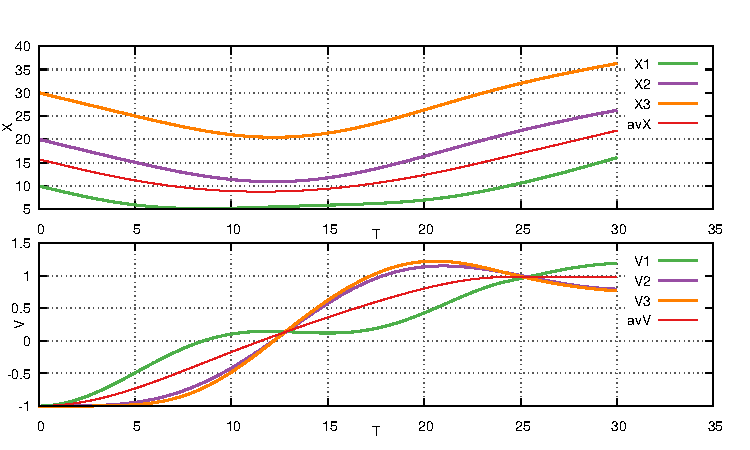
\includegraphics[width=1\textwidth]{tr/trbigm1m2.pdf} \\ б)
%        }
%    \end{minipage}
%    \begin{minipage}[h]{0.49\linewidth}
%        \center{
%           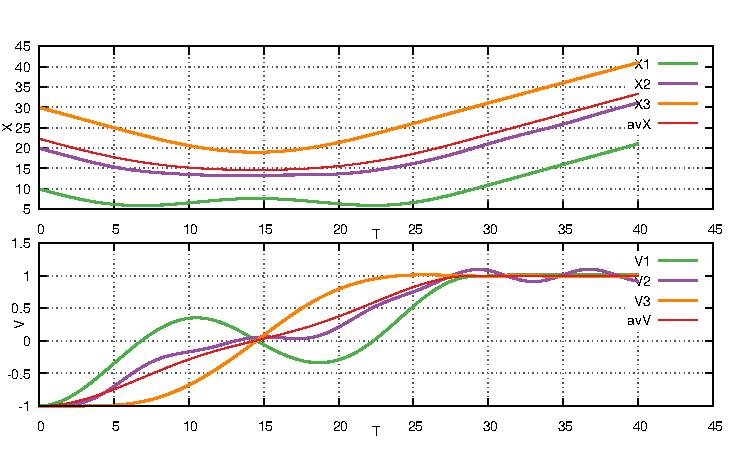
\includegraphics[width=1\textwidth]{tr/trbigm1m3.pdf} \\ в)
%        }
%    \end{minipage}
%    \begin{minipage}[h]{0.49\linewidth}
%        \center{
%           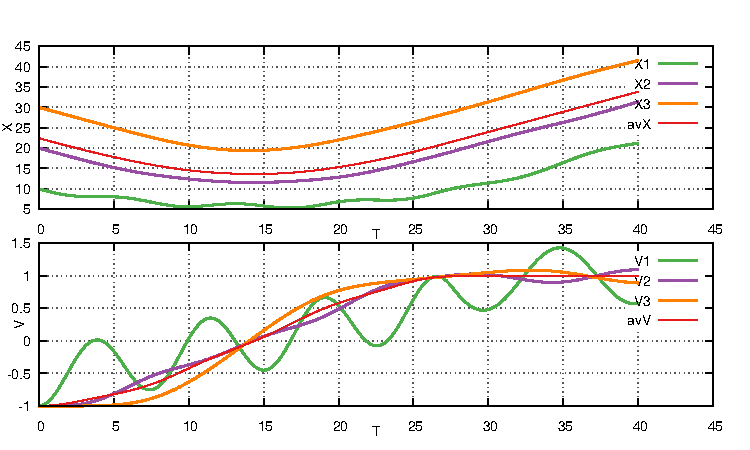
\includegraphics[width=1\textwidth]{tr/trbigm2m3.pdf} \\ г)
%        }
%    \end{minipage}
%    \begin{minipage}[h]{0.49\linewidth}
%        \center{
%           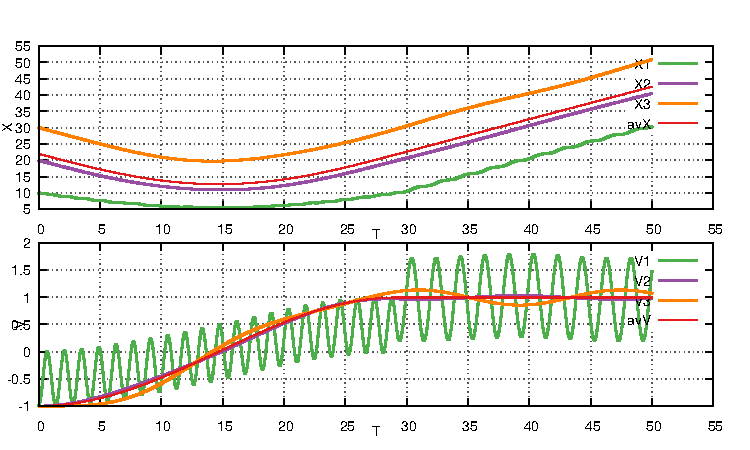
\includegraphics[width=1\textwidth]{tr/trmink.pdf} \\ д)
%        }
%    \end{minipage}
%    \caption{Траектории тела, при которых  $\Delta \tilde{E}$ минимальна. a) $m_1$ значительно больше остальных масс б) $m_1>>m_3$, $m_2>>m_3$\\
%    в) $m_1>>m_2$, $m_3>>m_1$, г) $m_2>>m_1$, $m_2>>m_3$, д) $k_1 \rightarrow 0$ }
%    \label{fig:mintr}
%\end{figure}
%
%
%\begin{figure}[t!]
%    \centering
%    \centering
%    \begin{minipage}[h]{0.49\linewidth}
%        \center{
%           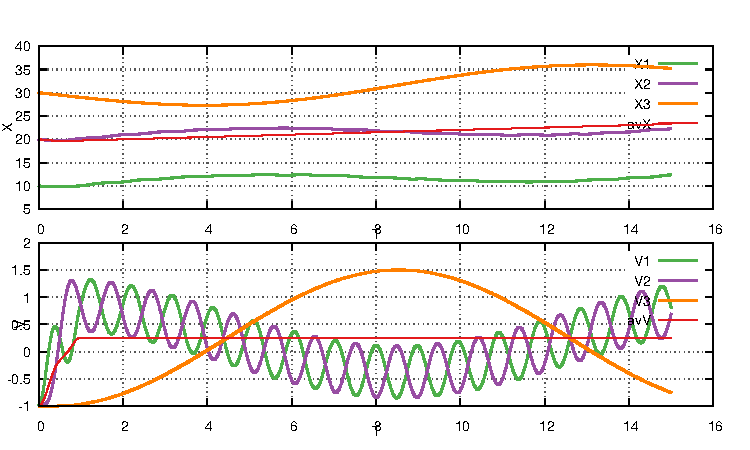
\includegraphics[width=1\textwidth]{tr/trmaxstfs.pdf} \\ a)
%        }
%    \end{minipage}
%    \begin{minipage}[h]{0.49\linewidth}
%        \center{
%           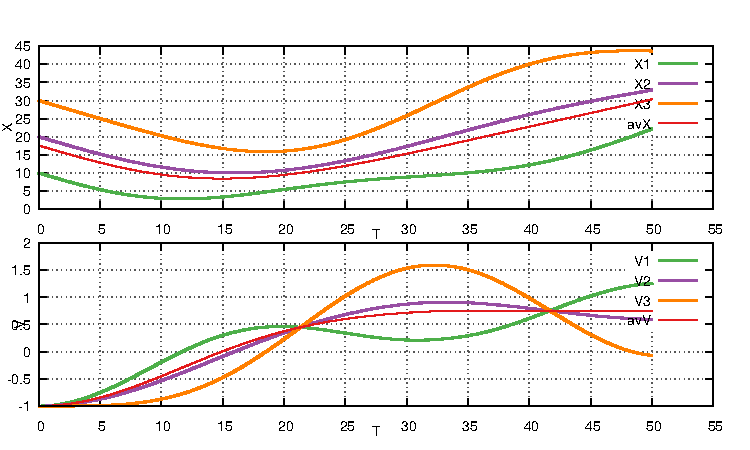
\includegraphics[width=1\textwidth]{tr/trlilm2.pdf} \\ б)
%        }
%    \end{minipage}
%    \caption{Траектории тела, при которой  $\Delta \tilde{E}$ максимальна а) для переменных жесткостей б) переменных масс}
%    \label{fig:maxtr}
%\end{figure}
%

На основе рисунков \ref{fig:mintr} и \ref{fig:maxtr} можно сделать вывод, что в предельных случаях система трех тел сводится к системе двух тел.
Значение диссипации будет зависеть от того каким образом система из трех тел преобразуется в систему двух тел при взаимодействии. 

Для максимума накопленной энергии система преобразуется в систему двух тел, в которой одно тело представляет из себя два тела, которые совершают гармонические колебания относительно общего
центра масс. Данный центр масс в свою очередь будет колебаться относительно оставшейся массы. Такая конфигурация позволяет преобразовать наибольшее количество
кинетической энергии тела на макроуровне во внутреннюю энергию тела.

В случае минимума наколенной энергии система стремится к единому абсолютно упругому телу, такие конфигурации сводятся к случаям, когда одна масса является
максимальной и вклад от других масс не является значительным. Так же есть случаи когда две массы совершают гармонические колебания, но третья масса является 
столь незначительной, либо засчет жесткости пружин не может внести достаточного вклада в данную систему. 
